
\section{Git and GitLab}

During your time at school or college, you'll no doubt have written essays and assignments that took more than one session to complete, and you've probably experienced some annoyances associated with transferring the files containing your work between different machines. Perhaps you started writing on a PC at college, took it home to work on a bit more, and finished it off in a library or on a laptop in a cafe. You may have moved the file around using a cloud-based system like Dropbox or Google Drive, or perhaps you transported it around with you on a USB drive. In any case, it's more than likely that at some point you'll have got yourself muddled up working out which version of the file is the latest, or needed to undo some changes and had to remember which version of the file to go back to. If you've been unlucky, you may have lost important changes along the way, or got to a stage where it feels impossible to undo some unwanted change that you've made because it affects so many different parts of your work that you don't know how to remove their effects without messing up your whole document. If you've ever tried to work collaboratively on a project with someone else, you'll probably have found it quite hard to co-ordinate changes so that things you do don't trample on things that someone else is working on at the same time. 

These are all well-known problems associated with doing any kind of writing or project work that takes more than a few minutes to complete, where you're using multiple machines and/or are working with other people; and as you work on more complex projects over longer periods of time and with bigger groups, the bad news is that these problems all get worse. You can, to a certain extent, improve the situation by sticking to certain conventions, such as making regular backups of your work with particular kinds of filenames, or promising always to email your collaborators before you make a change to anything and emailing them again when you've finished your changes. But these informal `social agreements' easily collapse when you are tired or stressed, leaving you with a mess to clear up. The good news is that there are industry-standard ways of dealing with these problems, this session we're going to introduce you to the basics of version control using Git and GitLab. 

`Git' and `GitLab' are tools to help you manage change. Whether you're working on something on your own or as part of a team, a little effort spent learning how to use these tools now will save you significant amounts of pain and hassle later on. 

Git is a version control system, and is one of the most popular of the thirty or so different systems in use today. It is arguably one of the most powerful and flexible version control systems available, and this does mean that your first contact with it can be a little daunting; but if you follow our instructions carefully and don't get too hung up on the bits that we're having to skim over to keep things simple, you'll soon get the hang of things. 

GitLab is a web-based interface to git which makes it easy (at least, easier) to set up projects and teams for collaborative work. Mastering any version control system takes a long time, and you may find in the early days that using git feels as though it's more hassle than it's worth---but version control is a crucial skill for any modern computer scientist, and it's important that you get used to the principles right from the start of your degree. And trust us, at some point it is going to save you an enormous amount of trouble!

In combination git and GitLab provide mechanisms for:
\begin{itemize}
\item Safely moving files from one machine to another without losing changes in the process. You'll probably find this useful early on, and essential when you start working on your group project.
\item Tracking changes that you've made so that you can safely undo things that you later decide you don't want.
\item Keeping things under control when you're working with others on a shared piece of work.
\item Exploring the content of projects via a friendly web interface.
\end{itemize}

Today we're going to keep things as simple as possible, and are just going to use git and GitLab for some simple version control and for moving files between machines.

Before we can start to use the tools properly, there's some housekeeping that we need to do. 

\section{Configuring git}

Git has already been installed on the School's PCs, but you'll need to set up some things that are specific to you, before it will work sensibly. 

Fire up a terminal, and enter the following commands one by one:

\begin{ttoutenv}
\$ git config --global user.name '[YOUR NAME GOES HERE]'
\$ git config --global user.email '[YOUR UNIVERSITY EMAIL ADDRESS GOES HERE]' 
\end{ttoutenv}

Hopefully the purpose of these commands is self-explanatory; you're just telling git who you are and how to contact you by email if it needs to. The next bits of configuration are a bit more mysterious, and explaining them in detail would take up way more space than we have here; for now we'll just say that they set the default way in which git interacts with GitLab:

\begin{ttoutenv}
\$ git config --global push.default simple
\$ git config --global branch.autosetuprebase always 
\end{ttoutenv}

The next few instructions are optional, but make the output of git nicer to read, so we recommend you also do:

\begin{ttoutenv}
\$ git config --global color.ui true
\$ git config --global color.status auto
\$ git config --global color.branch auto 
\end{ttoutenv}

and finally you should configure git to use whatever editor you've decided is your favourite at the moment, for example:

\begin{ttoutenv}
\$ git config --global core.editor nano 
\end{ttoutenv}

Check that you've typed these correctly by using the command \ttout{git config --list}. You should see all the things you've entered just now, along with a few other bits of default configuration that were set automatically for you by the system (you can safely ignore these for now).

\section{Setting up GitLab}

Next we're going to set up GitLab. Point your browser at the School's installation of GitLab at:
\\
\url{http://gitlab.cs.man.ac.uk}
and, on the `UoM Login' tab, log in with your University credentials. You should see GitLab's `dashboard' page and not much else (see Figure \ref{figure:GitLab-first-login}). Go to the `My Profile' section of GitLab using the icon at the top right of the page, and fill in any details about you that you're comfortable sharing with other students and staff within the School. At a minimum you should make sure that your Name and Email are set correctly; the other fields are optional. If you'd like your GitLab account to have an avatar image, you'll need to sign up for a \wikipedia{Gravatar}{Gravatar} account, which is a bit of a nuisance but not that hard.

\begin{figure}
\centerline{\includegraphics[width=15cm]{images/GitLab-first-login}}
\caption{First login to GitLab. \protect\circled{1} The GitLab logo (a sort of raccoon thing) will bring you back to the dashboard; useful if you get lost in GitLab's structure; \protect\circled{2} the user-profile allows you to add more information about yourself, and optionally connect up to Gravatar to give you a user icon; and \protect\circled{3} various ways to create a new project.}\label{figure:GitLab-first-login}
\end{figure}

\begin{diversion}{What about GitHub?}
You may have heard of a popular online git repository called GitHub, and be wondering why we don't just use that for your University work. GitHub is a fantastic resource, and is ideally suited for Open Source projects where you have lots of collaborators working together on a piece of Open Source code. GitHub's business model is that any project hosted on it must be Open Source, and visible for all users to see (not necessarily to edit). And of course, putting your solutions to lab exercises online for all to see is pretty-much the opposite of what we want to happen most of the time! It is possible to get non-open GitHub repositories set up, but GitHub quite reasonably charge for this service, and although it's possible to get non-open accounts for academic use, we decided it was cleaner to use our own installation of GitLab for Computer Science work, since we can hook it into the same authentication mechanisms that are used to control login to your other University services. The vast majority of features that you'll learn to use in GitLab can be easily transferred to other systems such as GitHub.
\end{diversion}

\section{Making your first project}

Git and gitlab both refer to collections of files that are being managed as `projects', because the most common case is that you are using them to control a software development project of some kind. There's no restriction on the size of a project really---it can have thousands of files in it, or just a few---and the layout of a project can mirror the kind of hierarchy that you'd have in your filestore, so you can have files and directories arranged however you like. We'll start off simple, and create a small project that represents the simple website you made in your previous lab sessions. Most version control systems use the term \concept{repository} to refer to the place where you store your files and the history associated with them. 

\begin{diversion}{Repositories}
Many version control systems such as \wikipedia{Subversion}{Subversion} have the idea of a central repository where you put your stuff, and from which you take copies of your files when you want to modify them. Git is rather different and is an example of what is called a \wikipedia{Distributed_revision_control}{Distributed Version Control} system; in the world of git you can have as many repositories as you like, each of which has a complete history of all the changes you've made. Instead of uploading and downloading from a central place, git has mechanisms to keep your repositories synchronised. 

In this case, however, we're using GitLab as a kind of `central repository' for your stuff. There's nothing special about the repository that GitLab manages from git's point of view really, except that we've set it up on a central server that's visible on the internet, so you can connect to it from anywhere using your University login details.
\end{diversion}

Select the `New Project' button from the icons at the top right (the one that looks like `+' symbol). Enter \fname{aboutme} as the project name, and hit `Create project'. You'll see a page similar to Figure \ref{figure:GitLab-new-project}. Notice that the `Git global setup' section contains the commands that you used in the previous section to set up your git configuration; so you don't need to do that again. There are also two other sections of code on how to `create repository' or use `Existing Git Repo?' (`Repo' is a common abbreviation for repository). Ignore both of these for now and instead follow the instructions here (we'll come back to them later in this session). Notice at the top of the GitLab page a warning that `You won't be able to pull or push project code via SSH until you add an SSH key to your profile'---we need to fix that first. Click on the `add an SSH key' link (marked with \protect\circled{1} on Figure \ref{figure:GitLab-new-project}), which will take you to the SSH key upload page which looks something like Figure \ref{figure:GitLab-ssh}.

\begin{figure}
\centerline{\includegraphics[width=15cm]{images/GitLab-new-project}}
\caption{Creating a new project in GitLab. \protect\circled{1} You will need to use the  `add an SSH key' link to upload your public key before you can communicate between git and GitLab, and the URL given in \protect\circled{2} can be used from the command line to clone and push this project.}\label{figure:GitLab-new-project}
\end{figure}

\begin{figure}
\centerline{\includegraphics[width=13cm]{images/GitLab-ssh}}
\caption{Adding a SSH key to GitLab. Once you have used \ttout{ssh-keygen} to create the key, paste the text into the `Key' box; if your key is valid then the title will be filled in for you.}\label{figure:GitLab-ssh}
\end{figure}

You'll now need to set up a means of securely identifying yourself to GitLab from whichever machine you're using at the time; this is done by creating what's called a \concept{SSH key}. In a terminal, type:

\begin{ttoutenv}
\$ ssh-keygen -t rsa -C '[YOUR UNIVERSITY EMAIL]'
\end{ttoutenv}

to create yourself a SSH key. When prompted `Enter file in which to save the key' just press return to accept the default, and the same for `Enter passphrase' twice.  For now don't worry too much about exactly what a SSH key is---we'll just treat it as a way of identifying yourself to the GitLab server. 

Look in a directory called \verb!~/.ssh! and you'll find two new files have been created called \ttout{id\_rsa} and \ttout{id\_rsa.pub}. The first of these is the \textit{private} part of the SSH key that's just been generated for you, and you should keep this secret. The second of these is the \textit{public} part of the key, and this is the bit you need to hand over to GitLab for it to be able to identify you. Use the command

\begin{ttoutenv}
\$ cat ~/.ssh/id_rsa.pub
\end{ttoutenv}
% $
to display the contents of your public key. You should see something like:

\begin{ttoutenv}
  
  ssh-rsa  AAAAB3NzaC1yc2EAAAADAQABAAABAQDTfAF0KxG94oUJLUER5Ci5HaoEtdi8KI0S+
  iro3EvVkQebW2V3nCaCLAHLmgmINm/NFW5bvbUq7bu2CxFlVBEQqa1idZBLceXKRi1SFtG+
  EzFENyzZBsIDU0IhfQX4qyxgqe0A3ortyAwm2/+0neu74RT0YK3gQI+wyxsFFoCzbahiDJisK
  /vKmqvwowb/Rrl3OZpX9ZO3QA9lgILLVy3J4VpAhR+05MyuM/Bzh/pYk5NIQivedUEduIJXLOetj/
  UnxlH9WbEPEIiDPvzrkb3xI98rLRSlh2hH89nc1SUfVEhY62RQWN7sbXPu+fFck7Dom9wE/
  YAG66Dbl30OsmFh mister.noodle@manchester.ac.uk

\end{ttoutenv}

which starts with \ttout{ssh-rsa}, ends with your email address, and has a load of apparently random characters in between. Select this text (making sure you don't accidentally select any extra newlines or spaces either side of it) and 
Copy and Paste the whole of the SSH key into the `Key' box on the GitLab page. If you've done this correctly, GitLab will spot the email from your key and use this as the `Title' field, in which case just press the Save button. GitLab will complain if it's not a valid key or has extra spaces or newlines at this point; if you're stuck here grab a demonstrator to help you. 

Once you've uploaded your public key to GitLab, you're ready to put your first bit of content into the `aboutme' project that you've just created. 

Click on the GitLab logo at the top left of the GitLab page to get back to the dashboard, and select the `aboutme' project that you created a moment ago. 

You now need to add some content to the project to play with, so go back to a terminal window. If you happen to have copied the web pages that you created about yourself from the introductory labs onto your desktop machine, you're welcome to use those for the rest of this session; just make sure they are \emph{not} in a directory called \fname{aboutme} right now (rename the directory using \ttout{mv} if they are). Otherwise, use \cmnd{curl}{curl} to fetch the sample `mrnoodle' webpages again (these are the ones that you experimented with on your Pi).

The URL for these is 

\url{http://studentnet.cs.manchester.ac.uk/ugt/COMP10120/files/mrnoodle.tar.gz}

and you will need to use \cmnd{tar}{tar} to `untar' this bundle of files using the command

\begin{ttoutenv}
\$ tar xvzf mrnoodle.tar.gz
\end{ttoutenv}

This will create a directory called \fname{htmlexample2}. 

Next we are going to \concept{clone} the (empty) project called \fname{aboutme} that you created in GitLab a moment ago onto your local filestore. Use the \cmnd{git}{git clone} command

\begin{ttoutenv}
\$ git clone [REPO-URL-GOES-HERE]
\end{ttoutenv}

replacing [REPO-URL-GOES-HERE] with the full URL (it will start with \texttt{ssh} rather than the more common \texttt{http}) that you can see at the top of your GitLab \fname{aboutme} project page, which is marked \protect\circled{2} in Figure \ref{figure:GitLab-new-project}. The URL will look something like:

\begin{ttoutenv}
ssh://gitlab@gitlab.cs.man.ac.uk:22222/mrnoodle/aboutme.git
\end{ttoutenv}

but obviously yours will be slightly different, so don't just cut and paste this one!

At this point, git will connect to GitLab, and make a copy of the empty \fname{aboutme} project in your filestore, creating you a copy of the project's repository. It should complete with the message `warning: You appear to have cloned an empty repository.' This is fine, because we know it's an empty repository at this stage.

\begin{diversion}{Connecting git to GitLab}
We could have set up our new project a different way, by initialising the project in our home directory (using \ttout{git init}) and then connecting that up to GitLab, but the later step of connecting a newly init'd repository with a project you've made in GitLab is a little fiddly, so it's slightly easier to explain what's going on the way we've done it here. We'll do it the `other way round' by starting with a directory full of files and sending that to GitLab later on in today's session. 
\end{diversion}

Change into the newly created \fname{aboutme} directory, and use \cmnd{ls}{ls -a} to see what's in there. It should be an empty except for a \concept{hidden directory} called \fname{.git}, which is where git is going to put its own administrative files. Feel free to take a look inside the \fname{.git} directory if you're interested, but please make sure you don't modify anything in there, otherwise you may get into a mess later on. 

Now copy the files from \fname{htmlexample2} (or your own website's directory) into \fname{aboutme/}. If you're using the default Mister Noodle ones, you'll have three files: one HTML, one .jpg and one .png (of course if you're using your own files, these may be different). 

Before we start adding these files to the project, let's see what git thinks the current status of that directory is. Use the \cmnd{git}{git  status} command 

\begin{ttoutenv}
\$ git status
\end{ttoutenv}

and you'll see a message from git that, amongst other things tells you that there are `untracked files' (these should appear in red). 

So we need now to tell git which files we want it to track for us. We need to \cmnd{git}{git add} \emph{each of the files in that directory} like this:

\begin{ttoutenv}
\$ git add [FILENAME]
\end{ttoutenv}

% $

replacing [FILENAME] with each of the file names in turn. Once you've done this, run \ttout{git status} again, and this time you should see that there are a list of `Changes to be committed' and all the files that you'd just added should appear in green. 

Now git knows which of the files in this directory you want to track (which in this case is all of them), we want to do our first \concept{commit}, which tells git that we've made a set of changes that we want to keep together: in this case the `changes' are to create the files in the first place; later on we'll go through a similar pattern of \ttout{git add} and \ttout{git commit} whenever we've done a set of changes that we think we are happy with. 

The \ttout{-m 'Initial Commit'} part of the commit line gives git a label to associate with this particular commit, and it's traditional to put the message `Initial Commit' the first time you tell git about a new set of files. In future you'll be putting text here that summarises in human-readable form what changes you've made in this commit, but more on that later.

\begin{ttoutenv}
\$ git commit -m 'Initial Commit'
\end{ttoutenv}

Don't worry about what git's response means here, that will become clear as you learn more. Type \ttout{git status} once again and if everything has gone to plan you should see the response

\begin{ttoutenv}
# On branch master
nothing to commit (working directory clean)
\end{ttoutenv}

If you get a different message here, then something has gone wrong in one of the previous steps; don't worry, just call a demonstrator to help out. 

So to recap: in GitLab we've created a project repository called `aboutme' ready to accept some files, and we have then \concept{cloned} this empty repository into your home directory (essentially making an exact copy of it). We then created some files in our local directory, used \ttout{git add} to tell git that we wanted to track them, and then \ttout{git commit} to tell git that those files in their current state form a sensible collection. 

Use the web-browser to go back to your \fname{aboutme} project page on GitLab. You'll see that nothing has changed on the server yet; that's because \ttout{git add} and \ttout{git commit} only make changes to the git repository \emph{that's on your local machine}.

The next step is to send a copy of these files to the GitLab server for safe keeping, and so that you can fetch them back from, say, your home machine. In git terminology, synchronising changes \emph{from} one repository (in this case your local one) \emph{to} another (in this case the one hosted on the GitLab server) is called a \concept{push}. 

Doing this is simple; just type:

\begin{ttoutenv}
\$ git push
\end{ttoutenv}

from within the \fname{aboutme} directory, and git will connect to your GitLab account, and copy the files and their revision history over on to the server for you (git knows where the files should go, because it's remembered where you got them from in the first place by storing that information somewhere in the hidden \fname{.git} directory you saw earlier, so you don't need to keep reminding it). 

Refresh your browser's GitLab project page again, and this time you should see a message saying that you have `pushed a new branch' (don't worry about the use of the word `branch' here---it's a reference to the fact that git can cope with multiple sets of changes happening in parallel and coming from different places). If you're not seeing that, summon a demonstrator to get help. 

If you now look at the `Files' menu in GitLab's page for your \fname{aboutme} project, you should see all the files that you added, committed and pushed; clicking on the individual file names should show you their content, so you can see what their latest status is. 

Look at the header of the table that contains your files, where it says `Name', `Last Update' and `Last Commit', and next to the `Last Commit' you will see a string of characters containing letters and numbers; this is a unique string that identifies your commit, and you can use it later to revert files back to the state they were in when you did that particular commit. Note that some times you'll see longer versions of this string (for example later when you use the \cmnd{git}{git log} command; as long as you give git enough characters for it to be able to uniquely identify a particular commit that you've made, git will be happy. So usually you don't need to use the long version).

Back at the command prompt, fire up an editor and make a small change to the HTML file; it doesn't really matter what the change is as long as it is something you can recognise as being different from the original version.

Then type \ttout{git status} again, and you'll see that git knows that you have modified that file since your last commit. Lets say that you want to remember this change next time you do a commit; you need to tell git this using 

\begin{ttoutenv}
\$ git add [NAME OF THE FILE YOU CHANGED]
\end{ttoutenv}

so do this, and then run \ttout{git status} once more to check that git now knows that you want it to remember the changes to this file since the last commit. 

It's important to understand that you need to run \ttout{git add} whenever you want git to recognise a change you've made to a file; if you make changes \emph{after} having run \ttout{git add}, git will not take those into account unless you run \ttout{git add} again to tell it that you really did mean to make those changes. You don't have to do it after every edit; just after edits that you want to keep. 

In git terminology, this process is called \concept{staging}; think of it as `setting the stage' or `getting things ready' to be put into your project's history. 

But for now, let's assume that this is the only change you need to make right now, and that you want  git to remember this change as part of your project's history; the command for this is called \cmnd{git}{git  commit} Type

\begin{ttoutenv}
\$ git commit -m '[SOME WORDS THAT DESCRIBE YOUR CHANGE]'
\end{ttoutenv}

replacing the text in braces (and the braces themselves) with something that would help you remember what you did if you needed ever to check in future. 

At this stage, your change has been recorded in the \emph{local} git repository in your filestore. To push this change over onto the GitLab server, you just need to type

\begin{ttoutenv}
\$ git push
\end{ttoutenv}

once more, and everything will get synchronised with your GitLab account.

Go back to the GitLab page for this project in your browser, and look at the status of the project's files now and you should see this change reflected there. Notice now that the unique identifier for your Last Commit has now changed, and that whatever comment you put in on the commit line also appears in the table to remind you where you're up to. 
Notice also that only the file you modified has been updated; the others will still say `Initial Commit' against them, since nothing will have changed there since your first commit. 

Experiment a bit now by editing the files again (perhaps use the Gimp application to change the images as well as editing the HTML file), and practise using \ttout{git add}, \ttout{git commit} and \ttout{git push} to record these changes and send them to the GitLab server. At each stage, use \ttout{git status} to confirm that git is reporting what you'd expect it to, and look again at the GitLab page in your browser to make sure that makes sense at each step too. 

When you're happy that you understand these three commands, you're ready to move on to the next step.

\section{Keeping files synchronised between two repositories}
Imagine now that you've gone back home and want to retrieve the latest files you've been working on. Don't go back home though, there's still more work to do in the lab! 

In git terms, what you want to do is to get a copy of your project repository on your home machine. For now we'll simulate that by just making a new directory in your CS filestore, and cloning your project into there. 

In your home directory make a new directory called \fname{gittest}, and \ttout{cd} into it; we're going to use this to pretend that you're now in a different machine that can't see your computer science filestore directly. Assuming that you've got git installed, and have a SSH key on your home machine, the process would be identical.

Use the same \ttout{git clone} command that you used earlier to get yourself a \emph{new copy} of your \fname{aboutme} project from GitLab; you should then find a copy of \fname{aboutme} has appeared in your current working directory. Unlike previously where \ttout{git clone} created an empty directory for you (because you'd not put any files into the project at that stage), you should now find that this new \fname{aboutme} contains the latest versions of the files from your other version of the project.

Use the \cmnd{git}{git log} command to see what the history of this project is; you should see all the commits that you've made so far, along with the descriptions gave for what the commits meant. 

Make another change to one of the files, then \ttout{add}, \ttout{commit} and \ttout{push} that change to the GitLab server's repository. Check that you can see these latest changes in the GitLab web pages.

Go back to your \emph{original} \fname{aboutme} directory (imagine that you're now back at the University doing some work in the lab, and want to pick up the changes you made to your stuff when you were at home). This time you want to do the opposite of a \ttout{push} in order to bring your local copy up to date with whatever is on the server. The command to achieve this is called, not unreasonably, \cmnd{git}{git pull}, so run that now, and you should find that you once more have an up-to-date version of your work. Hurrah!

Practice making changes in one or the other of the two \fname{aboutme} directories that you've made (imagining that one of them represents a directory on your machine at home), and make sure you're comfortable with the cycle of using \ttout{add}, \ttout{commit} and now both \ttout{push} and \ttout{pull} to move changes `between machines' via the GitLab server.

\section{Reverting a file to a previous version}

Let's say you've messed one of your files up in a recent change, and want to go back to a previous version. You need to find the unique number that's associated with the commit that had the version you want. Use \ttout{git log} to see your change history and pick one of the commits that you've made already (your comments should tell you what you did in that commit; if they're not helpful, you might want to think about what kind of comments you're using!). Find the long number associated with that commit, and type

\begin{ttoutenv}
\$ git checkout [UNIQUE NUMBER FOR COMMIT] [NAME OF FILE YOU WANT TO REVERT]
\end{ttoutenv}

If you've got this right, git will just return you to the command prompt without complaining; if you get an error or warning that you don't understand, grab a demonstrator. 

Look at the file you've just checked out, and you should see that it's one of the old versions you had previously. You've now got the choice of continuing to work with the file you've just reverted (you'll need to \ttout{add} it back later before doing a commit), or throwing it away and picking another version. If you want to discard it and get back to the latest version of that file, just use \ttout{git checkout HEAD [NAME OF THE FILE]} to get back to the most recent edits (here `HEAD' just means `the most recent version that I've committed').


\section{A Recap}

Before moving on to do some `real' stuff with git and GitLab, let's quickly revisit some of the key ideas.

\begin{enumerate} 
\item When you're working with git, the files and directories that you're editing are held locally in your filestore just like any other files or directories. In git terminology this local copy is called your \concept{workspace} or \concept{working copy}. 
\item When you first want to tell git to track a file fore you, or after you've modified a file with a change that you want git to later remember when you do a commit, you use the \cmnd{git}{git add} command to \concept{stage} the file. This records the current status of the file temporarily in what is called the \concept{staging area} (or is sometimes referred to as the \concept{index}). The content of staged files only get recorded in the project's history the next time you run \cmnd{git}{git commit}. 
\item When you want to record a set of changes together, you use the \cmnd{git}{git commit} command, which takes any staged files and records their state in the \concept{local repository}, and the commit message in the project's log.
\item If you want to synchronise your local repository with another repository elsewhere (referred to as the \concept{remote repository} or more correctly as the \concept{upstream repository}), you can either \cmnd{git}{git pull} changes \emph{from} the upstream repository, or \cmnd{git}{git push} them \emph{to} the upstream repository. In our case, we're using GitLab as your upstream repository.
\end{enumerate}


\subsection{The lifecycle of a file under git's control}

It's also important to be clear about the \emph{lifecycle} of a file that's being looked after by git. This is illustrated in Figure \ref{figure:git-file-life-cycle}. A file \protect\circled{1} will start off life being \concept{untracked}, i.e. it's a file that git knows nothing about. Using the \cmnd{git}{git add} command, you can ask git to track the status of the file, at which point the file is \concept{staged} \protect\circled{2}. You can them \cmnd{git}{git commit} this file, and any others that have been staged, which makes a copy of them in the project's local repository, and returns their status to being \concept{unmodified} \protect\circled{3} because now the file's content is in sync with the version you've just committed. Editing the file causes it's state to change to \concept{modified} (i.e. `not the same as what's in the latest commit') \protect\circled{4}; and you can use \cmnd{git}{git add} to put the file back in the staging area ready to commit again. This cycle is repeated until the project is finished. 



\begin{figure}
\centerline{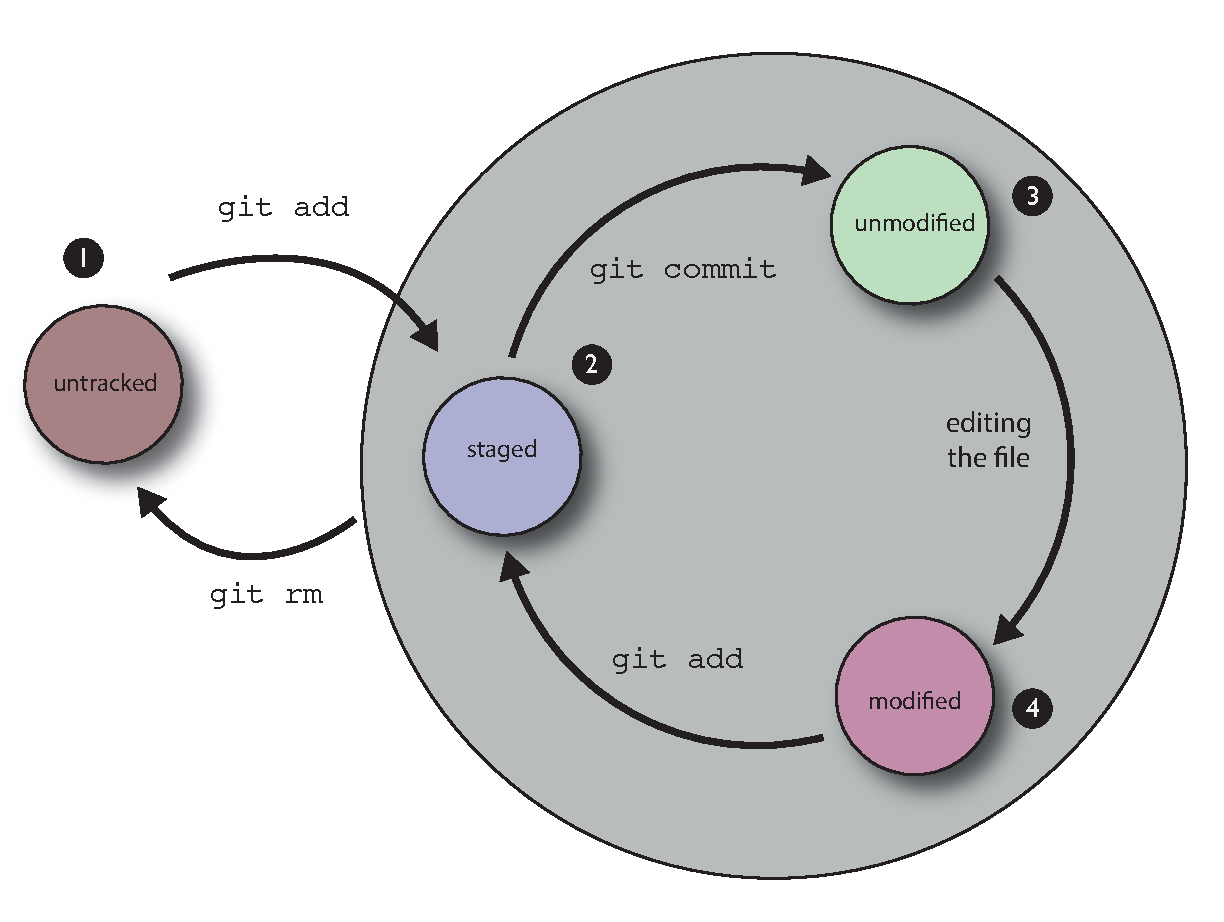
\includegraphics[width=15cm]{images/git-file-life-cycle}}
\caption{The life cycle of a file under git's control.}\label{figure:git-file-life-cycle}
\end{figure}

You should now have enough knowledge to be able to do three things with git and GitLab.

\begin{enumerate}
\item Use them together to safely move files between different machines, knowing that your content will be backed up in GitLab, and also that the history of changes that you've made will get preserved nicely.
\item Use GitLab as a handy way of looking at the content of files in your project (for example, if you only have access to a web browser and not a machine with a command-line interface).
\item Use git to safely revert files to previous versions if you've got yourself into a pickle. 
\end{enumerate}

Git and GitLab together can do much more than this, and will be invaluable tools when you start to use them for your group project work. But it's important right now that you just get into the habit of using them on your own to manage your own individual work; it'll make the few extra things that you will need to learn to use them as a group-tool much easier.

And yes, you'll probably think that using git is more hassle than just shoving all your stuff into a cloud based system and hoping for the best; but please trust us, by practising this stuff now you're not only developing an essential skill for your future careers, you will find at some point soon that it saves you a lot of pain and hassle. 


\subsection{Basic git commands again}

\begin{figure}
\centerline{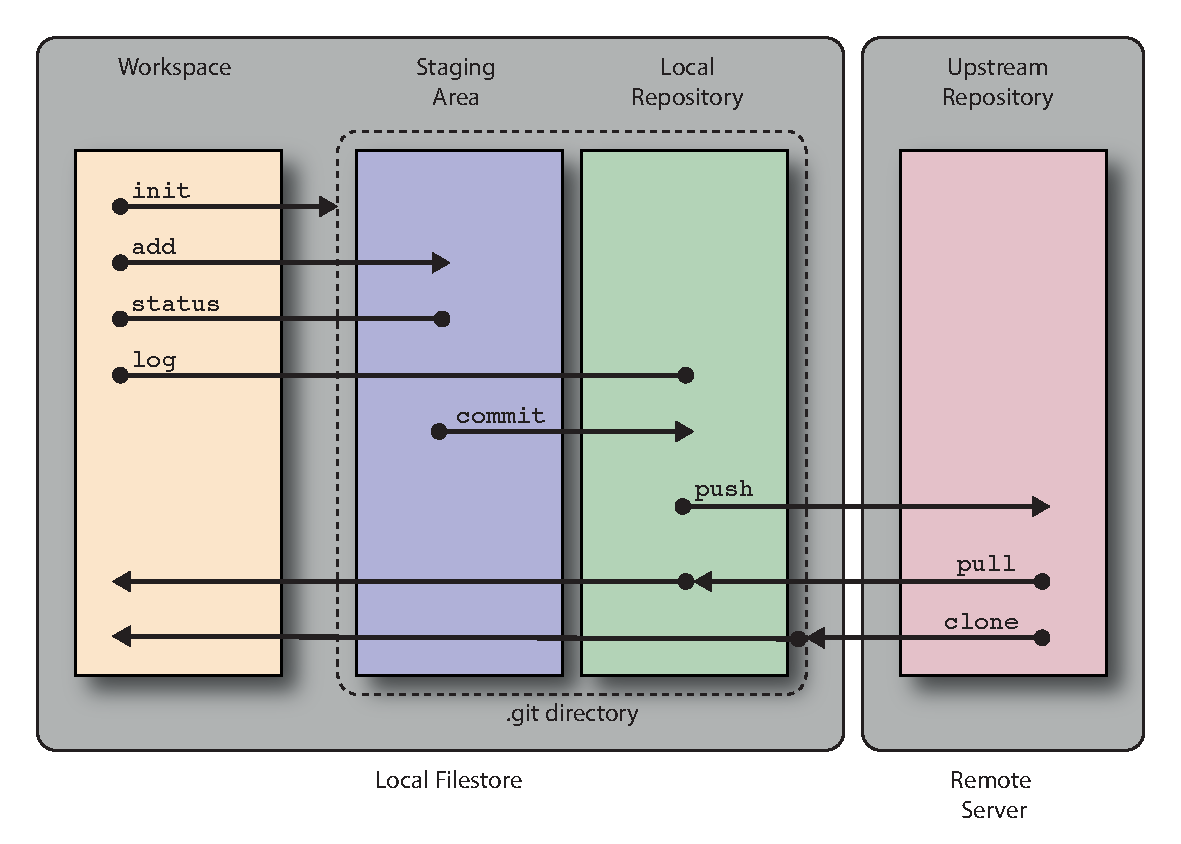
\includegraphics[width=15cm]{images/git-commands}}
\caption{Basic git commands and their interaction with the various repositories}\label{figure:git-commands}
\end{figure}

Figure \ref{figure:git-commands} shows how the various commands we've looked at so far interact with the different repositories used by git. 

\begin{itemize}
\item \ttout{git init} creates an empty local repository in the current working directory. 
\item \ttout{git add} `stages' a file by adding the \emph{current content} of new or modified files to the staging area. 
\item \ttout{git status} gives you the status of files in the workspace and staging area. It will tell you which stage of the file life cycle (Figure \ref{figure:life-cycle} each file is in. This command doesn't know anything about the status of any upstream repositories.
\item \ttout{git log} gives you the commit history of your project, giving you the unique identifiers and messages associated with each commit.
\item \ttout{git commit} bundles together all staged files, and commits them to the local repository along with a message describing the change. Remember, this doesn't automatically push your changes to the upstream repository, it's only makes the changes locally. 
\item \ttout{git push} updates the upstream repository with any commits that have happened since the last push. If the upstream repository has changed in the meantime (for example, because someone else has pushed new changes before you), this command will fail with an error to prevent you accidentally over-writing something else.
\item \ttout{git pull} fetches the latest changes from the upstream repository, and merges them into the local one, updating the workspace versions in the process.
\item \ttout{git clone} downloads a repository from a server.  
\end{itemize}


\exercisess{Recording your progress so far}

In your \fname{COMP10120} directory, create a new subdirectory called \fname{ex4}. In your \fname{aboutme} directory, run the \cmnd{git}{git log} command, and redirect its output to a file called
\begin{ttoutenv}
\fname{\$HOME/COMP10120/ex4/aboutme.gitlog}
\end{ttoutenv}
 using the command  
\begin{ttoutenv}
\$ git log > \$HOME/COMP10120/ex4/aboutme.gitlog
\end{ttoutenv}

Then change into the \fname{ex4} directory and check that the contents of \fname{aboutme.gitlog} is what you expect. This file is one of the things that \ttout{submit} will pick up when you run it at the end of the lab sessions; the \emph{exact} contents of the file don't matter, but we will expect it to show the history of your \fname{aboutme} project, and to have some sensible commit messages. 

\section{Putting real work into git}

So far we've experimented with some throw-away webpages in your \fname{aboutme} directory. Now it's time to put some real content into git and GitLab.

\exercisess{Putting \fname{COMP10120} under version control}

Make a new project in GitLab called \fname{COMP10120}. 

This time, because you already have some content that you want to put into a project (rather than starting `from scratch' like we did earlier), go to your \fname{COMP10120} directory and type \ttout{git init}. This should respond by saying that it has `initialized empty Git repository'. Now look through the different files and directories that are in \fname{COMP10120}, and use \ttout{git add} to add \emph{only those files that you want git to track for you}. What's important here is that you only add files that are your original source files (for example, those that end with .tex), and not things which are automatically generated by tools such as the .pdf or .aux files created by LaTeX.

Use \ttout{git status} regularly to check that the files you want to track, and \ttout{only} the files you want to track have been added to git's list, and then use \ttout{git commit} to make your initial commit. 

Next you'll want to synchronise your local repository with the one in GitLab. This is a little more fiddly than just doing a `clone' like we did earlier, but just follow these instructions and all will be well.
 
Look back at the aboutme project's page on GitLab, and find the \fname{COMP10120} project's URL (again, this is labelled with \protect\circled{2} in Figure \ref{figure:GitLab-new-project}).

Then enter the following command, copy-and-pasting the URL from the web page into the appropriate bit of command line:

\begin{ttoutenv}
\$ git remote add origin [GitLab-URL-GOES-HERE]
\end{ttoutenv}

This makes an association between the repository that you've created in your filestore, and the project in GitLab.

Finally to send this first version of the repository over to the GitLab server, enter

\begin{ttoutenv}
\$ git push -u origin master
\end{ttoutenv}

which should respond with some variation of 

\begin{ttoutenv}
Counting objects: 3, done.
Writing objects: 100% (3/3), 216 bytes, done.
Total 3 (delta 0), reused 0 (delta 0)
To ssh://GitLab@GitLab.cs.man.ac.uk:22222/mister.noodle/aboutme.git
 * [new branch]      master -> master
Branch master set up to track remote branch master from origin by rebasing.
\end{ttoutenv}
 
Check using your browser that GitLab has now received the right versions of your files for the \fname{COMP10120} project.

Use the same output redirection mechanism we used a moment ago to record the output from \ttout{git log} for the \fname{COMP10120} project into a file called \fname{COMP10120.gitlog} in your \fname{COMP10120/ex4} directory so that \ttout{submit} can find it later. Once again, the \emph{exact} contents of the file don't matter as long as it is a sensible representation of your commit history for this project.

If this has worked, then move on to the final exercise. If there are any problems, or you're at all unsure about what's going on, find a demonstrator to help you. 

\exercisess{Putting your \fname{COMP16121} exercises under version control}

To finish off this laboratory session, create a project for \fname{COMP16121} and put all the appropriate files under git's control. Remember again -- you only want to put \emph{source} files or files that you've created yourself into git, not ones that are the output of the Java compiler or any other program.

Now this time there are probably a lot more files to worry about, and you might not want to go through them one by one \ttout{git add}ing them each individually. Instead you could use something like this to add them to the staging area:

\begin{ttoutenv}
\$ cd ~/COMP16121
\$ git add ex*/run-all-tests
\$ git add ex*/task*/run-tests
\$ git add ex*/task*/*.java
\end{ttoutenv}

Check that only the files you want to add have now been staged using \cmnd{git}{git status}, and get help from a demonstrator if the result isn't what you expected.

When you're happy that the staged files are the correct ones, use \ttout{git commit} to commit them, and then save the git log to a file called \fname{COMP16121.gitlog} in your \fname{COMP10120/ex4} directory (this is your final submittable deliverable for today's session). 

When your Java code is all safely in GitLab and you have three log files recorded in \fname{COMP10120/ex4}, you're done for today (but if you have a machine that you can use at home, please take the opportunity to see if you can clone the projects you've made today onto that to experiment further). 


\section{Using Git for real}

It's really important that you're comfortable with basic git usage, and you should make sure that from now on any work that you do in \emph{any} of the labs (not just in COMP10120) is put under git control. This will make it much easier for you to work on files from home, and may also get you out of trouble if you get carried away with the \cmnd{rm}{rm} command at some point, because you will have some backup stored in GitLab (every year, someone will accidentally delete important work; don't be that person---put everything you do in GitLab and you can't go too far wrong!)

\section{Other git learning resources}

Git is widely documented and discussed online, and there are loads of excellent resources that you can use to improve your understanding of  source code control systems generally, and git specifically. In particular:

\begin{itemize}

\item Schott Chacon's `Pro Git' book is available online for free and is an excellent guide to git from the very basics to much more advanced use than is covered in today's lab session. It is well worth a read and is at \url{http://git-scm.com/book}

\item There's a very useful quick-reference site at \url{http://gitref.org}

\item Andrew Peterson's Interactive Git Cheat Sheet is also a very useful reference tool, though probably only makes sense when you are reasonably familiar with git. It's located at \url{http://ndpsoftware.com/git-cheatsheet.html}
\end{itemize}

\section{Git `Best Practice'}

These are some basic principles that you should keep in mind when you're using git (or any version control system, really). They are very much \emph{principles} rather than rules; things that you should aspire to do unless there are very good reasons not to. On the whole sticking to these means that you'll be able to use source code control systems more effectively, and will avoid some of the pitfalls that can trap you if you're careless. 

\begin{enumerate}
\item \textbf{Commit \emph{related} changes}. A commit should really represent one conceptual change to your work. This may (and probably will) involve changes in several files, but ideally you should be able to describe what the commit means in a single sentence. For example, if you are fixing more than one bug, you should probably be doing more than one commit. If you find that the message you'd be putting into the log to describe the change involves the word `and', you may want to think again (for example, a change that `fixes the startup bug, and improves the colour scheme in the logo' should really be two separate commits). The universe won't grind to a halt if you do this, but it does mean that in future it would be harder to change your logo colour without undoing the startup bug fix as well.

\item \textbf{Commit frequently} Making lots of smallish commits helps avoid the problem described above, and also makes it easier to undo changes if you find something bad has happened. 

\item \textbf{Avoid committing half-finished things}. Try to make sure that when you do a commit it represents exactly one fully finished change; a commit that's only half a change is much harder to describe in a commit message, and harder to understand later when you come back to your work. This is especially important when you are working in collaboration with other people; a half-working (which of course means half-not-working!) commit means that your collaborators get a broken system to work with, and that won't make you popular.

\item \textbf{Write meaningful commit messages}. Its tempting sometimes to abbreviate or put junk into your commit messages to save hassle at the point of committing, but this will come back to bite you later; your collaborators will not appreciate this at all either. Ideally the first line of your message should be a short (around 50 character) description of the change, so that it can fit onto a single line of a terminal when you look at the log. You can then add a blank line, followed by a more comprehensive description of what changes you've made (why did you make this change? how is it different from before?)


\end{enumerate}

\section{Marking Scheme}

\markschemeurl{4}

















